\documentclass[a4paper,12pt]{article}
\usepackage[english,ngerman]{babel}
\usepackage[utf8]{inputenc}
\usepackage{times}
\usepackage{amsmath}
\usepackage{amssymb}
\usepackage{amsfonts}
\usepackage{amsthm}
\usepackage{graphicx}
\usepackage{fancyhdr}
\usepackage{textcomp}
\usepackage[all]{xy}
\usepackage{txfonts}
\usepackage{array}
\usepackage{makeidx}
\usepackage{verbatim}
\usepackage{pdflscape}
\usepackage{paralist}
\usepackage{epic}
\usepackage{hyperref}
\usepackage{geometry}
\geometry{papersize={210mm,297mm},total={160mm,240mm},top=31mm,bindingoffset=15mm}
\setlength{\unitlength}{1pt}
\usepackage{color}
\begin{document}
\title{Anleitung zum Mathematischen Seminar}
\date{}
\maketitle
\section{Einleitung\label{einleitung}}
Im Rahmen des mathematischen Seminars schreiben Sie eine Seminararbeit
zu einem mathematischen Thema.
Dabei geht es in erster Linie darum, ein mathematisch/naturwissenschaftliches
Argument zu erarbeiten und auszuformulieren.
Sie arbeiten zu zweit an Ihrem Thema, Sie arbeiten aber auch 
innerhalb des gr"osseren Seminar-Projektes, welches als Ziel das
Seminar-Buch hat.

Sie sind daher auch nicht ganz frei in der Wahl der Werkzeuge, die Sie
zur Formatierung der Seminararbeit verwenden, und erst recht nicht
in der Art und Weise, wie Ihr Beitrag Eingang ins Gesamtprojekt findet.

Die Wahl dieser Werkzeuge ist Ihnen bereits abgenommen worden.
Sie ist weder willk"urlich noch durch pers"onliche Vorlieben diktiert,
sondern entspricht dem Standard in Mathematik und Physik und vielen
technischen Wissenschaften.
Viele Zeitschriften in diesen Gebieten erwarten Manuskripte typischerweise
formatiert in \LaTeX, und auch an der HSR ist seine Verwendung 
vor allem im Studiengang E das Werkzeug der Wahl f"ur Studien- und
Bachelor-Arbeiten.

Die Zusammenarbeit der vielen Autoren wird vereinfacht durch das
Versionsverwaltungssystem GIT.
Es wurde urspr"unglich von Linus Torvalds f"ur die Verwaltung des
Source Code des Linux Kernel geschrieben.
Es hat sich aber mehr oder weniger zu einem Standard entwickelt,
moderne Projekte werden meistens mit damit verwaltet.

Die meisten Studierenden arbeiten im Mathematischen Seminar zum ersten
Mal an einem gr"osseren Dokumentationsprojekt zusammen, und kennen daher
diese Werkzeuge noch nicht.
Die folgenden Abschnitte versuchen, den Einstieg zu vereinfachen.
Sie beschr"anken sich auf das unbedingt N"otige.
Es gibt gen"ugend weiterf"uhrende Literatur, mit der Sie Ihre Kenntnisse
vertiefen k"onnen, und die allwissende M"ullhalde, das Internet,
bietet zahllose Quellen zur Vertiefung.
Von besonderem Interesse im Zusammenhang mit
\LaTeX\ \url{http://tex.stackexchange.com}.

\section{Die Seminararbeit\label{seminararbeit}}
In diesem Abschnitt werden ein paar Hilfen zur Gestaltung der Arbeit
mit \LaTeX{} zusammengestellt.

\subsection{Text}
Der Text ist nat"urlich der zentrale Teil Ihrer Arbeit, und auch der
Teil, wo sie im Team am erkennbarsten zusammen arbeiten k"onnen m"ussen.
Sie gehen aus von den bereits bereitgestellten Files \verb+main.tex+
und \verb+main.bib+ (f"ur das Literaturverzeichnis) im Unterverzeichnis,
das Ihrer Arbeit zugewiesen ist.

Ihren Text geben Sie als eine Mischung von reinem Text und sogenannte
Kontroll-Sequenzen oder Makros ein.
Die Makros erm"oglichen Sonderzeichen darzustellen, die im Textzeichensatz
nicht zur Verf"ugung stehen.
Bei der Verwendung von ASCII zum Beispiel ben"otigen bereits die Umlaute
"a, "o und "u
die Kontroll-Sequenzen 
\verb+"a+,
\verb+"o+ und
\verb+"u+.
Im Allgemeinen beginnen Kontrollsequenzen jedoch mit $\tt{\backslash}$.
Formeln im Text werden mit \verb+$+ eingerahmt, herausgestellte Formeln,
die auf einer eigenen Zeile stehen, sogenannte Displays, werden wie folgt
gesetzt:
\begin{verbatim}
\[
\int_{-\infty}^\infty e^{-x^2/2}\,dx = \sqrt{2\pi}
\]
\end{verbatim}
Der zugeh"orige Output ist
\[
\int_{-\infty}^\infty e^{-x^2/2}\,dx = \sqrt{2\pi}
\]
Es steht eine riesige Menge von Makros zur Darstellung so ziemlich
aller mathematischen Formeln zur Verf"ugung.
Sie k"onnen f"ur Ihre Zwecke zum Beispiel im Skript abkupfern, oder
die vielen Tutorials auf dem Internet konsultieren, oder mit Google
nach Hilfen suchen, die meistens auf Stackexchange f"uhren.

Hier noch ein paar Empfehlungen, die ihren Code lesbarer machen und
die Kollaboration vereinfachen:
\begin{itemize}
\item Jede Formel auf eine eigne Zeile. 
Erfahrungsgem"ass ist das Vorgehen bei "Anderungen am Text anders
als bei "Anderungen an Formeln, daher ist es sinnvoll, diese bereits
im Source-Code auseinander zu halten.
\item Jeder Satz auf eine neue Zeile. 
Da Kollaborationswerkzeuge typischerweise zeilenweise arbeiten,
k"onnen "Anderungen, die zwei verschiedene Autoren am Text machen,
nur dann wieder zusammengef"uhrt werden, wenn die beiden Autoren
verschiedene Zeilen ge"andert haben.
Wenn jeder Satz auf einer neuen Zeile beginnt, hat das zur Folge, dass
"Anderungen zusammengef"uhrt werden k"onnen, wenn sie verschiedene 
S"atze betreffen.
\item Ein neuer Absatz wird durch eine Leerzeile signalisiert, nicht
durch irgendwelche Makro-Aufrufe.
Insbesondere d"urfen Sie nicht durch \verb+\\+ einen neuen Absatz
einleiten.
Dieses Makro erzeugt nur einen Zeilenwechsel, \TeX{} betrachtet den
nachfolgenden Text als Teil des selben Absatzes.
Das ist zum Beispiel daran erkennbar, dass der "ublich Einzug am Anfang
eines neuen Absatz nicht erscheint.
\item Wenn die Trennung von \TeX{} nicht automatisch richtig gemacht
wird, dann f"ugen sie ``discretionary hyphens'' hinzu, eigentlich nur
Instruktionen an \TeX, wie ein Wort getrennt werden muss. 
Sie d"urfen keine festen Trennungsstriche einf"ugen, denn wenn der
Text umformatiert werden muss (zum Beispiel wenn aus drucktechnischen
Gr"unden das Seitenformat ge"andert werden muss), dann entstehen
pl"otzlich nicht getrennte W"orter mitten in einer Zeile,
die Bindestriche enthalten.
\item K"ummern Sie sich bei der Eingabe Ihres Textes nicht um die
Platzierung auf der Seite, dies ist die Aufgabe von \LaTeX.
Und wenn ihnen das optische Resultat nicht gef"allt, dann ist das nicht
Ihr Problem, sondern das Problem des Herausgebers des Seminar-Buches,
der f"ur die herausgeberische Aufarbeitung zust"andig ist.
\end{itemize}

\subsection{Bilder}
Ein Bild sagt mehr als tausend Worte.
Streben Sie also an, Ihre Erkenntnisse m"oglichst aussagekr"aftigen
Bildern zu illustrieren und verst"andlich zu machen.
Leider liefert die Google-Bildersuche nicht immer wirklich gute Bilder,
geben Sie sich also nicht damit zufrieden, suchen Sie Darstellungen,
die Ihre Ideen am besten ausdr"uckt.

Dies kann auch bedeuten, dass Sie eine graphische Darstellung selbst
erzeugen m"ussen.
Eine breite Palette von Softwareprodukten steht f"ur diesen Zweck
zur Verf"ugung, doch zeigt die Erfahrung, dass alle Produkte
eine gewisse "Ubung verlangen, bis gute Resultate entstehen.
In jedem Fall m"ussen Sie f"ur gute Resultate Zeit investieren.

Die Abbildungen des Skriptes sind zu einem bedeutenden Teil mit
Hilfe von Metapost erzeugt.
Metapost ist eine Graphik-Sprache, die aus dem Metafont-System abgeleitet ist,
mit dem die zu \TeX\ geh"origen Schriften erzeugt wurden.
Als Bestandteil jeder einigermassen vollst"andigen \TeX-Distribution
ist es eine naheliegende Wahl, wenngleich vielleicht nicht die einfachste.
Die M"oglichkeiten sind jedoch in vielen F"allen v"ollig ausreichend.
Sie k"onnen die Beispiele im Skript als Basis f"ur Ihre eigenen Entwicklung
nehmen.
Sehr viel vollst"andiger aber auch komplexer ist Tikz.

Was auch immer Sie verwenden, streben Sie an, dass die erzeugten Graphiken
Vektor-Graphiken sind, damit sie bei jeder beliebigen Aufl"osung
optimal dargestellt werden.
Bei Buchdruck werden sehr viel h"ohere Aufl"osungen verwendet als
beim Laserdruck, Pixelgraphiken k"onnen beim Laserdruck akzeptabel
aussehen, bei h"oheren Aufl"osungen werden die Defizite sichtbar.
JPG Bilder sind also dann zweckm"assig f"ur photographische Bilder.

Zudem sollten Sie in Ihren Bildern Transparenz vermeiden, da gewisse
Druckmaschinen damit Schwierigkeiten haben. Der PDF-Standard, der
in der Druckvorstufe "ublich ist, ist deutlich "alter als was von
\LaTeX{} erzeugt wird.

\subsection{Literaturverzeichnis}
Jede Seminararbeit hat ihr eigenes Literaturverzeichnis.
Um die Formatierung der einzelnen Eintr"age brauchen Sie sich nicht
zu k"ummern, auch dies "ubernimmt \TeX.
Sie m"ussen aber die bibliographischen Angaben in strukturierte
Form bereitstellen. 
Dies geschieht im File \texttt{main.bib} im Verzeichnis ihrer
Seminararbeit.
Nehmen Sie die Beispiele im File \texttt{references.bib} als
Vorlagen, weitere Informationen k"onnen Sie auch auf Stackexchange finden.

\subsection{Pr"asentation}
Ihre Erkenntnisse sollen Sie auch in einer Pr"asentation ihren Kollegen
vorstellen.
In der Wahl Ihrer Pr"asentationsmittel sind Sie frei, doch das Sie
bereits bereits f"ur Ihre Seminararbeit \LaTeX\ eingesetzt haben, 
liegt es einigermassen nahe, dasselbe Werkzeug auch f"ur die Pr"asentation
zu verwenden.
Dies erlaubt Ihnen Graphiken und Formeln direkt wieder zu verwenden.

Meistens wird f"ur Pr"asentationen das \texttt{beamer}-Package 
verwendet.
Im Internet finden Sie viele Beispiele oder sogar Vorlagen f"ur
seinen Einsatz, die Sie f"ur Ihre Zwecke adaptieren k"onnen.


\section{Werkzeuge\label{werkzeuge}}
Eine Implementation der nachstehend beschriebenen Produkte f"ur
Ihre bevorzugte Plattform finden Sie im Internet.

\subsection{Texteingabe}
Die Wahl eines Editors ist eine sehr pers"onliche Sache, sie hat
viel mit den eigenen Arbeitsgewohnheiten zu tun.
Im Rahmen der Einschr"ankung von \TeX{} sind sie v"ollig frei in der
Wahl ihres Texteingabe-Werkzeuges.

Word oder ein anderes Office-Produkt ist allerdings genauso wenig
f"ur die Eingabe von \TeX-Code geeignet wie für die Erstellung von
Programmcode.
Es ist auch nur beschr"ankt der Versionierung und Kollaboration
zug"anglich, wie sie in diesem Projekt angestrebt wird.
Sie m"ussen daher einen Editor verwenden, der f"ur Programm-Code
geeignet ist.

Im FS17 wird erstmals mit utf8-Text gearbeitet, so wie er in Java
schon seit sehr langer Zeit "ublich ist.
Es ist daher darauf zu achten, dass utf8-Zeichen, insbesondere 
Umlaute und korrekt codiert und wiedergegeben werden.
Ist dies in Ihrem Editor nicht m"oglich, m"ussen die traditionellen
Zeichensequenzen zur Codierung von Umlauten und anderen Sonderzeichen
verwendet werden, also \verb+"a+ f"ur \texttt{"a}, \verb+"o+ f"ur
\texttt{"o}, \verb+"u+ f"ur \texttt{"u} usw.

Ausser gew"ohnlichen Text-Editoren stehen f"ur \TeX{} auch verschiedene
GUI-Tools zur Ver\-f"u\-gung, naturgem"ass sind da die pers"onlichen
Vorlieben aber noch wichtiger.
Leider sind diese GUI-Tools nicht alle gleich nützlich.
Insbesondere sind nicht alle gleich gut mit Versionierung und
Kollaborations-Tools vertr"aglich.

\subsection{Unix und Makefiles}
Einer Tradition folgend verwalte ich das Projekt auf Unix Systemen
(Linux und/oder Mac OS X).
Die Beschreibung der Befehle zur Versionsverwaltung zum Bau des
Skriptes beziehen sich auf die Unix/Mac Umgebung.
Sie sind aber in analoger Form auch f"ur Windows-Benutzer zust"andig,
ich bitte die ge"ubten Windows-User, die wichtigsten Unterschiede
als Hilfestellung zu diesem Dokument beizutragen, genau zu diesem
Zweck ist es Bestandteil des Github Projektes.

In der Unix-Umgebung ist naheliegend, die Verwaltung der Abh"angigkeiten
mit dem immer vorhandenen Werkzeug \texttt{make} vorzunehmen.
Die Makefiles beschreiben, wie die verschiedenen Produkte des Projektes
aus den Source-Files erzeugt werden m"ussen.
Es gen"ugt, im \texttt{skript}-Verzeichnis den Befehl \texttt{make} zu geben, 
worauf das Programm \texttt{make} das gesamte Skript neu baut.
Das \texttt{make}-Kommando leitet aus den Makefiles ab, was alles gemacht
werden muss, wenn einzelne Files ge"andert werden.
Windows-User m"ussen hier einen Extraschritt selbst gehen, und m"oglicherweise
einzelne Kommandos von Hand eingeben, um zu einem vollst"andigen Build
zu kommen.

Alternativ kann man sich auch eine virtuelle Maschine mit einem
Linux-Betriebssystem einrichten.
Moderne Linux-Distributionen enthalten alle Werkzeuge, die f"ur die
Formatierung des Buches n"otig sind, darin eingeschlossen die
Erzeugung aller Bilder.
Da nur einfach Textfiles editiert werden m"ussen, kann jeder beliebige
Text-Editor dazu verwendet werden, was auch relativ leicht zu erlernen ist.
Linux ist gerade auch im Bereich Embedded Systems weit verbreitet, so
dass eine gewisse Vertrautheit damit sicher keine Negativqualifikation ist%
\footnote{Die Elektrotechnik-Abteilung der ETH verwendet fast ausschliesslich
Linux.}.

\subsection{GIT}
Die \TeX-Files des Seminar-Projektes werden als Github-Projekt gef"uhrt,
Sie finden es unter \url{https://github.com/AndreasFMueller/Seminar17}.
Die sp"ater abgebildeten Screenshots stammen vom letzten Jahr und
verwenden daher das Projekt \verb+SeminarDGL+.
Es ist zwar jedermann m"oglich, auf die Files dieses Projektes zuzugreifen,
aber eigene Beitr"age zum Projekt k"onnen Sie so nicht leisten.
Sie sollten daher als erstes ein eigenes Account auf \url{https://github.com}
einrichten.

\subsubsection{Verzeichnis f"ur Ihre Arbeit}
In der File-Hierarchie des Projektes steht Ihnen ein eigenes Verzeichnis
f"ur Ihre Beitr"age zur Verf"ugung.
Sie finden es unter \texttt{skript/thema}, wenn \texttt{thema}
die Kurzbezeichnung Ihres Themas ist.
In diesem Verzeichnis befindet sich bereits ein File \texttt{main.tex}
mit einer Vorlage.
Sie k"onnen sofort beginnen, dieses File zu erweitern, oder sie k"onnen
von diesem File aus weitere Files einlesen (mit dem \verb+\input+
Befehl).
Ebenfalls steht bereits ein noch leeres File \texttt{main.bib} f"ur
das Literaturverzeichnis bereit.
Zu Ihrem Verzeichnis k"onnen Sie beliebige Files hinzuf"ugen, und
die darin vorhandenen Files jederzeit "andern.
"Anderungen an anderen Files d"urfen Sie jedoch nicht vornehmen, und als
Projektadministrator werde ich Pull-Requests (siehe weiter unten)
abweisen, die "Anderungen an Files anderer Projektteilnehmer vornehmen.

\subsubsection{Forking}
\begin{figure}
\centering
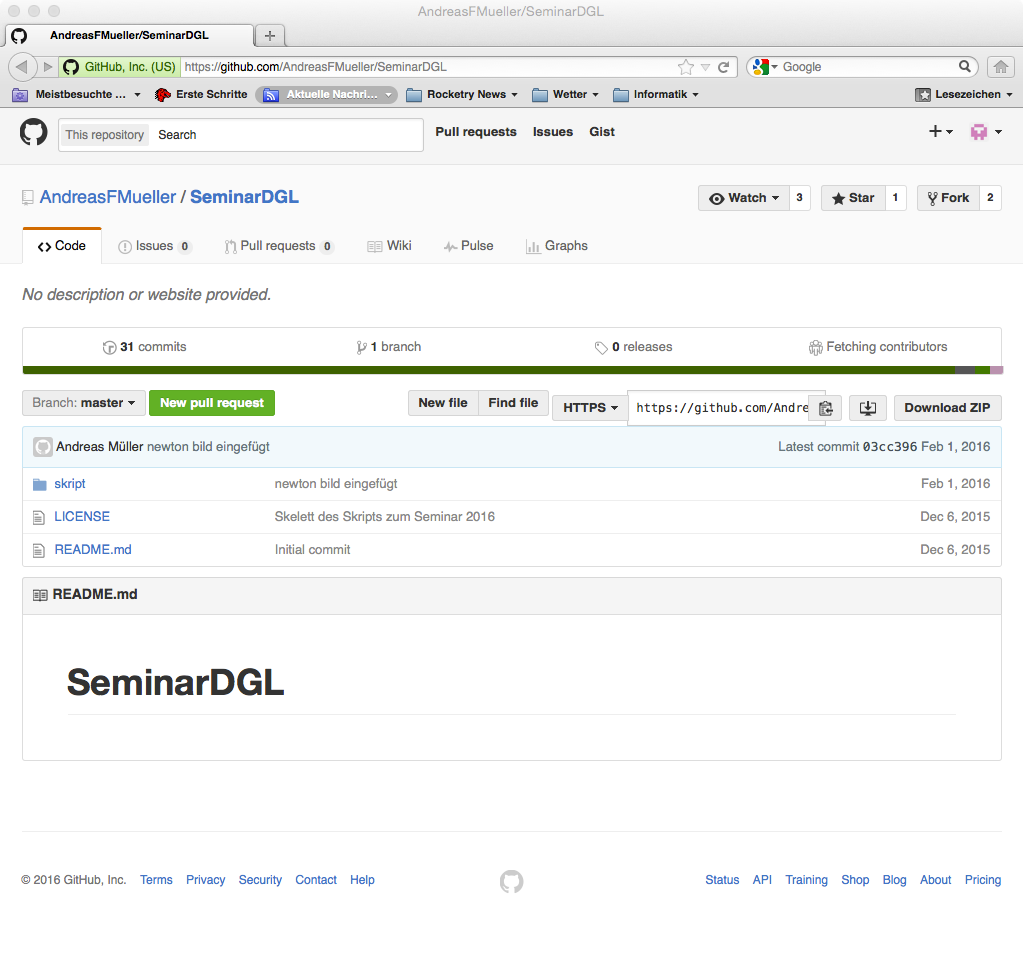
\includegraphics[width=\hsize]{fork.png}
\caption{Projekt \texttt{SeminarDGL} des Benutzers \texttt{AndreasFMueller},
bereit zum Forken durch den Benutzer \texttt{SeminarTeilnehmer}.
Forken erfolgt durch den Knopf {\bf Fork} in der rechten oberen Ecke.
\label{fork}}
\end{figure}
\begin{figure}
\centering
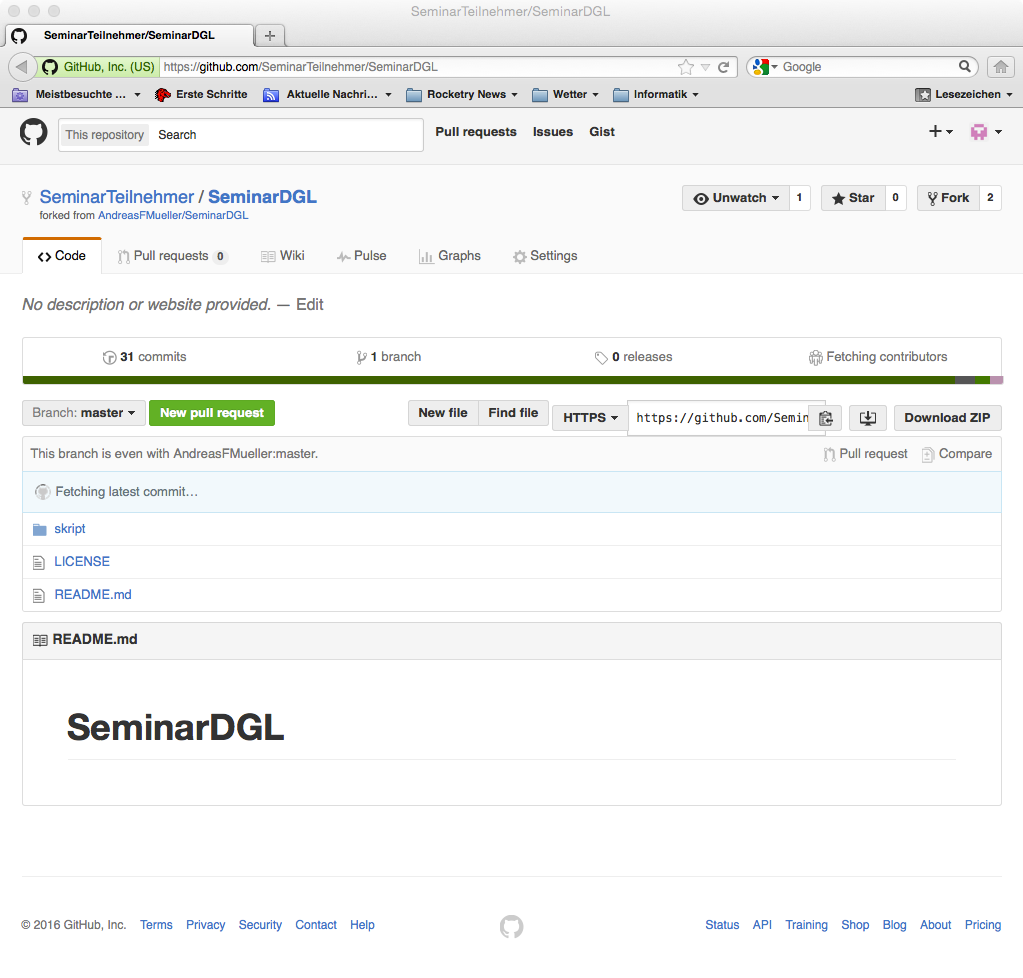
\includegraphics[width=\hsize]{forked.png}
\caption{Fork des Projektes \texttt{SeminarDGL} durch den Benutzer
\texttt{SeminarTeilnehmer}.
An dieser Kopie kann der Benutzer jetzt beliebige "Anderungen vornehmen.
\label{forked}}
\end{figure}
Bevor Sie "Anderungen an den Files vornehmen k"onnen, m"ussen Sie
einen Fork des Projektes erstellen.
Suchen Sie dazu das Projekt \texttt{SeminarDGL} des Benutzers
\texttt{AndreasFMueller}.
In der rechten oberen Ecke des Webinterfaces finden Sie einen Knopf
\textbf{Fork} (Abbildung~\ref{fork}).
Klick darauf erzeugt eine Kopie des Projektes in ihrem eigenen Account
(Abbildung~\ref{forked}).
In diesem Fork f"ugen Sie ihre Seminararbeit hinzu und bearbeiten
Sie, bis sie bereit ist, in das "ubergeordnete Projekt integriert
zu werden.

\subsubsection{Cloning}
Bevor Sie an den Files "Anderungen anbringen, brauchen Sie eine 
lokale Kopie des Projektes.
Sie erreichen das durch {\em Clonen}.
Der Befehl dazu ist
\begin{verbatim}
> git clone https://github.com/SeminarTeilnehmer/SeminarDGL.git
Cloning into 'SeminarDGL'...
remote: Counting objects: 236, done.
remote: Total 236 (delta 0), reused 0 (delta 0), pack-reused 236
Receiving objects: 100% (236/236), 253.56 KiB | 157.00 KiB/s, done.
Resolving deltas: 100% (143/143), done.
Checking connectivity... done.
\end{verbatim}


\subsubsection{Commit}
Ihre "Anderungen werden permanenter Bestandteil des Projektes durch 
den Commit.
Damit die anderen Projektteilnehmer verstehen, was Ihre "Anderungen
bewirken, verlangt der Commit eine kurze Beschreibung derselben.
Gew"ohnen Sie sich daher an, oft zu committen, damit die "Anderung
mit einem kurzen Statement beschrieben werden kann.

Es gibt zwar einen abgek"urzten Befehl \texttt{commit -a}, der einfach
alle "Anderungen committet, doch besteht dabei die Gefahr, auch
unbeabsichtigte "Anderungen aussehalb Ihres eigenen Teilbereiches zu 
Committen, und damit die Files anderer Projekttteilnehmer unbeabsichtigt
zu "andern.
Sie sollten daher alle Commits immer explizit f"ur die Files eingeben,
die Sie tats"achlich ge"andert haben, also zum Beispiel
\begin{verbatim}
> git commit einleitung.tex
\end{verbatim}
Sie werden dann dazu aufgefordert, einen Kommentar einzugeben. 
Sie k"onnen die Message aber auch gleich mit dem Befehl mitgeben:
\begin{verbatim}
> git commit -m "neuer Verweis auf Literaturverzeichnis" einleitung.tex
\end{verbatim}
Nach diesem Befehl finden Sie ein neues Verzeichnis \texttt{SeminarDGL}
auf Ihrem Computer, mit allen n"otigen Komponenten, um das Skript
neu zu bauen.
An diesen Files k"onnen Sie, mit den genannten Einschr"ankungen,
Ihre Arbeit einf"ugen und beliebig bearbeiten.

\subsubsection{Push und Pull}
Auch nach einem Commit sind Ihre "Anderungen im Repository noch nicht
sichtbar, sie sind erst lokal in Ihrem Projekt eingetragen.
Der Push-Befehl transferiert Ihre lokalen "Anderungen ins Repository,
sie werden damit f"ur alle sichtbar.
Sie arbeiten nicht allein, m"oglicherweise hat Ihr Partner "Anderungen
vorgenommen, die sie auch gerne sehen m"ochten.
Der einfachste Weg ist, diese "Anderungen zu ``Pushen'', damit sie
sichtbar werden.
Der Befehl dazu lautet
\begin{verbatim}
> git push
Password for 'https://SeminarTeilnehmer@github.com': 
Counting objects: 3, done.
Delta compression using up to 8 threads.
Compressing objects: 100% (3/3), done.
Writing objects: 100% (3/3), 417 bytes | 0 bytes/s, done.
Total 3 (delta 0), reused 0 (delta 0)
To https://SeminarTeilnehmer@github.com/SeminarTeilnehmer/SeminarDGL.git
   03cc396..3610eb4  master -> master
\end{verbatim}
Sie verwenden dann den Pull-Befehl, um die nun sichtbaren "Anderungen
in ihre eigene Kopie zu integrieren.

\subsubsection{Pull-Request}
\begin{figure}
\centering
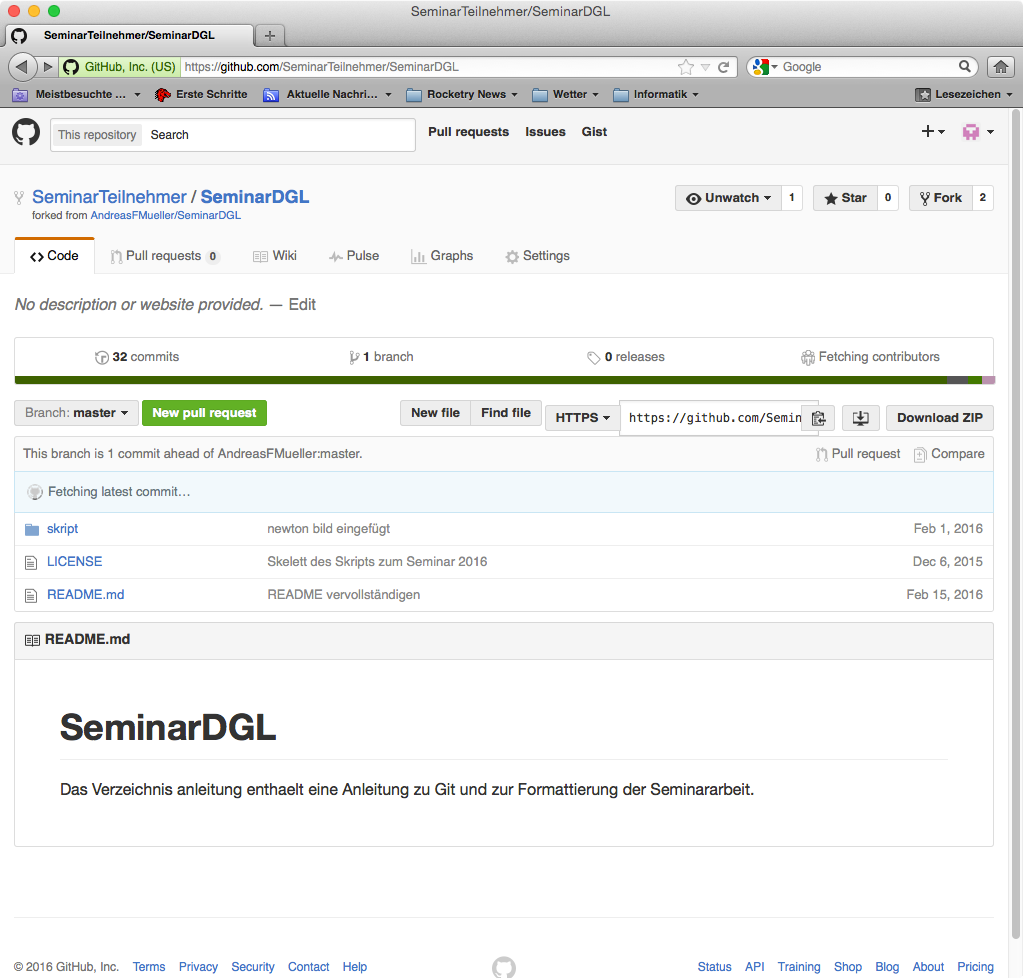
\includegraphics[width=\hsize]{newpullreqest.png}
\caption{Einen neuen Pull-Request erzeugen: Knopf {\bf New pull request}
klicken
\label{newpullrequest}}
\end{figure}
\begin{figure}
\centering
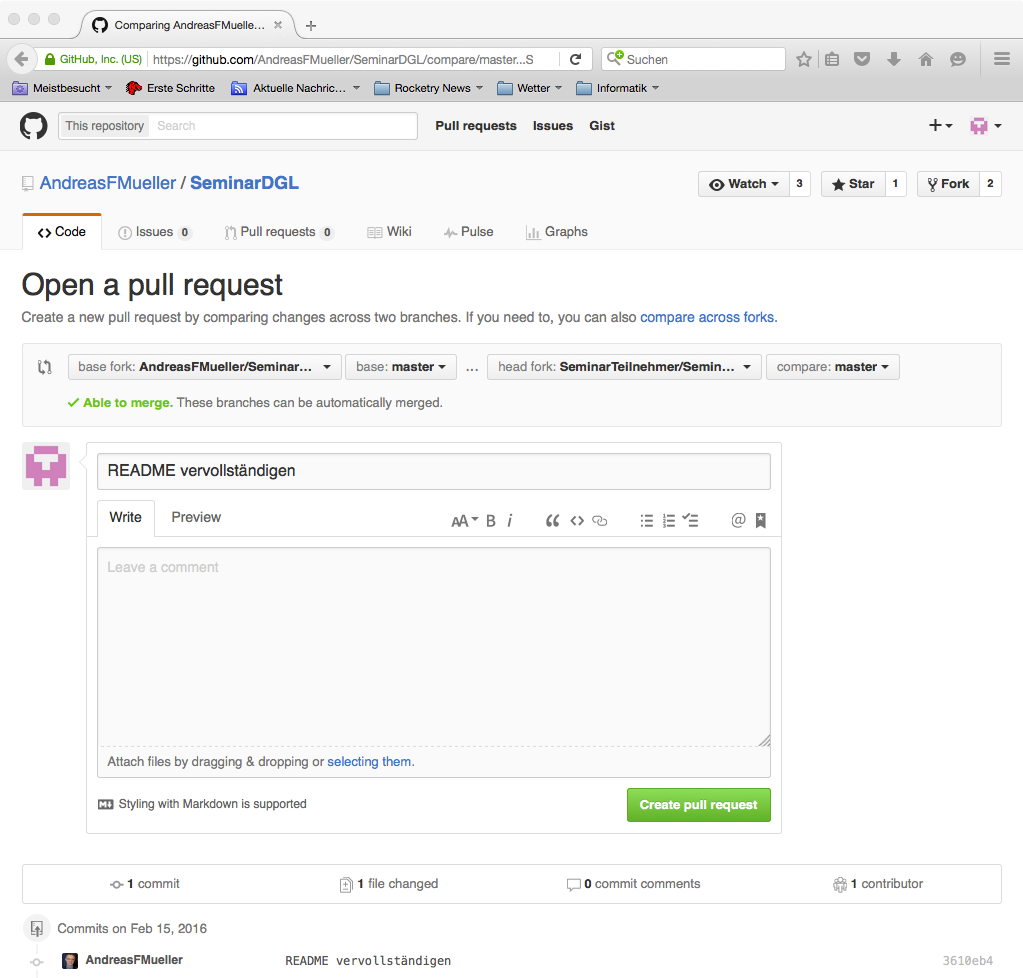
\includegraphics[width=\hsize]{openpull.png}
\caption{Github untersucht, ob der Pull-Request sinnvoll angewendet
werden kann, und erlaubt dem Benutzer, einen Kommentar dazu einzugeben.
\label{openpull}}
\end{figure}
\begin{figure}
\centering
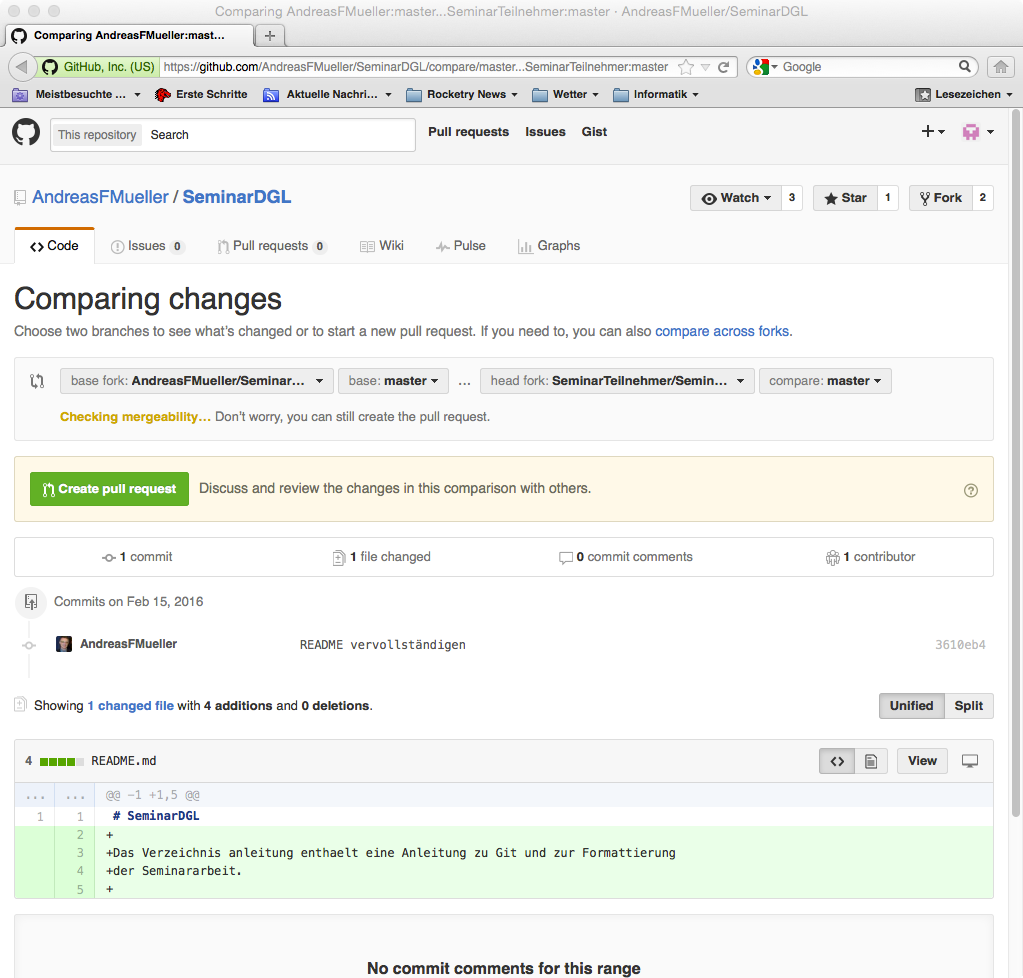
\includegraphics[width=\hsize]{preparepullrequest.png}
\caption{Github zeigt die Elemente, die im Pull-Request enthalten sind.
\label{pullresult}}
\end{figure}
%\begin{figure}
%\centering
%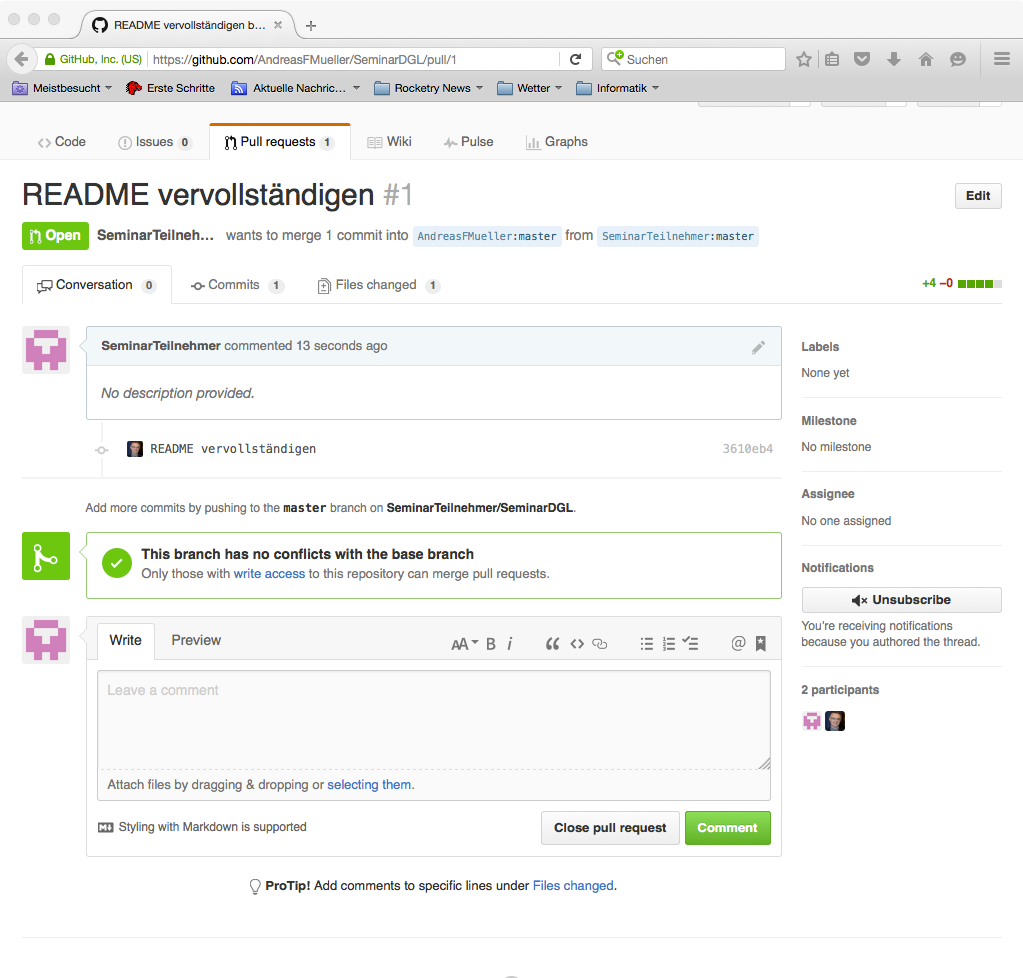
\includegraphics[width=\hsize]{pullresult.png}
%\caption{So pr"asentiert sich der Pull-Request dem Projekt-Administrator
%\label{pullresult}}
%\end{figure}
Am Ende m"ochten Sie Ihre Arbeit in das Gesamtprojekt integrieren.
Bis jetzt haben Sie an Ihrem eigenen Clone gearbeitet, der nicht f"ur
alle Seminarteilnehmer sichtbar ist.
Sie haben auch nicht das Recht, einfach so eine "Anderung vorzunehmen,
ich als Herausgeber des Seminar-Buches m"ochte meinen Senf dazu geben
k"onnen.
Sie m"ussen mir daher Ihren Beitrag mit Hilfe eines Pull-Requests
"ubermitteln.
Diesen k"onnen Sie direkt auf dem Github Webinterface erzeugen.
Ich werde ihn dann daraufhin kontrollieren, ob er die in diesem
Dokument beschriebenen Regeln einh"alt, und in das Projekt
integrieren.
Sie k"onnen auch nach dem Pull-Request weiter an Ihrem Dokument
arbeiten, Verbesserungen anbringen.
Nutzen Sie die Gelegenheit, schon fr"uh Feedback zu Ihrer Arbeit
einzuholen, so ist der Lerneffekt am gr"ossten.

Die Erzeugung eines Pull-Request ist in den Abbildungen
\ref{newpullrequest},
\ref{openpull}
und
\ref{pullresult} dargestellt.
In Abbildung~\ref{newpullrequest} sieht man den Knopf, mit dem der
Benutzer~\texttt{SeminarTeilnehmer} den Pull-Request anfordert.
Github untersucht dann, ob der Pull-Request "uberhaupt sinnvoll
erzeugt werden kann, und zeigt die Elemente, die der
Pull-Request enthalten wird (Abbildung~\ref{openpull}).
Der Benutzer kann dann eine Mitteilung eingeben, die dem Verwalter
des urspr"unglichen Projektes zu verstehen gibt, was der Pull-Request
beabsichtigt.
In Abbildung~\ref{pullresult} ist das Resultat des Pull-Request zu
sehen, wie ihn auch der Projektadministrator sieht.

\subsection{\LaTeX}
Das \TeX-System wurde in den Achtziger-Jahren von Donald Knuth entwickelt,
weil er mit der Satz-Qualit"at nicht zufrieden war, die der Herausgeber
seines Buches {\em The Art of Computer Programming} zu produzieren in
der Lage war.
Vor allem die Qualit"at des Formelsatzes war aus Knuths Sicht 
ungen"ugend.
Knuths System wurde von der Mathematikern und Physikern sehr rasch
aufgenommen und weiterentwickelt, besonders in Form des Makropakets
\LaTeX\ hat es sich zum Standard f"ur technische Dokumentation
entwickelt.

\subsubsection{Markup}
Im Gegensatz zu einem Wysiwyg System wie Microsoft Word verwendet
\TeX\ den Markup-Ansatz.
Der Autor eines Dokumentes k"ummert sich ausschliesslich um den Inhalt,
er "uberl"asst die graphische Darstellung "uberl"asst er dem System.
Der Input besteht daher aus reinen Text-Files, die neben dem eigentlichen
Text einzelne Instruktionen enthalten, die \TeX\ mitteilen, ob es sich
bei dem Text um einen Titel, eine Bildunterschrift, oder eine Fussnote
handelt.
F"ur die Unterteilung des Textes in Abs"atze ist "uberhaupt
kein spezieller Markup n"otig, eine leere Zeile signalisiert
dem \TeX-System den Anfang eines neuen Absatzes.
Insbesondere ist es falsch, einen Zeilenumbruch mit Hilfe eines
doppelten Backslash zu verlangen.

Markup bedeutet auch, dass die Darstellung jederzeit an ver"anderte
Bedingungen angepasst werden kann.
Vielleicht muss das Buch bei einem anderen Drucker hergestellt
werden, was eine "Anderung des Seitenformats zur Folge haben kann.
Daher d"urfen keine Markup-Instruktionen verwendet werden, die die
sich nur auf Aussehen oder Layout beziehen.
Zum Beispiel ist es nicht zul"assig zu verlangen, dass eine Abbildung
an einer ganz bestimmten Stelle auf der Seite erscheint, denn mit
anderen Seitenabmessungen k"onnte diese Anweisung nicht mehr sinnvoll
sein.

%F"ur mathematische Formeln steht eine sehr reichhaltige Palette von
%Markup-Befehleen und Makros zur Verf"ugung, die auch automatische
%alle Konventionen der mathematischen Typographie einhalten.
%So sind zum B eispiel Variablen wie $x$ oder $y$ oder Funktionen wie
%$f(x)$ oder $g(y)$ immer in einer schr"agen Schrift gesetzt, w"ahrend
%trigonometrische Funktionen wie $\sin x$ und $\cos \alpha$ aufrecht
%geschrieben werden.
%Der einfachste Weg, mit den M"oglichkeiten vertraut zu werden,
%ist die Beispiele des Skriptes als Vorlage zu nehmen und f"ur die
%eigenen Bed"furfnisse anzpassen.Bed"urfnisse anzpassen.

%Da Markup keine Information "uber die Darstellung enth"alt,
%empfiehlt es sich, vor allem auf gute Editier- und Lesbarkeit
%des Source-Code zu achten.
%Zum Beispiel soll jede Seite einer Gleichung auf einer eigenen
%Zeile stehen, ode sogar jeder einzelne Term.

\subsubsection{Packages}
Packages fassen zusammengeh"orige Markup-Makros zusammen.
Eine breite Auswahl f"ur das Skript n"otiger Packages werden durch
das Haupt-File \texttt{skript.tex} bereits eingelesen.
Leider lassen sich nicht alle Package mit jedem anderen Package
kombinieren, ausserdem verl"angern viele Packages die Zeit, die
\TeX\ braucht, um das Skript zusammenzubauen.
Sollten Sie f"ur die Darstellung Ihrer Resultate ein Package ben"otigen,
welches noch nicht eingebaut ist, kl"aren Sie bitte erst ab, ob Sie
Ihr Ziel auch mit einem vorhandenen Package erreichen k"onnen.
Falls nicht, f"ugen Sie das Package zu \texttt{skript.tex} hinzu,
und kontrollieren Sie, ob dadurch kein Konflikt in anderen Seminararbeiten
entsteht.
L"asst sich das Skript immer noch erfolgreich bauen, k"onnen Sie das
neue Package in \texttt{skript.tex} Committen und in ihrem Pull-Request
dem Projekt hinzuf"ugen.

\end{document}
